\documentclass[handout, t]{beamer}
\usepackage[latin1]{inputenc}
\usepackage{pgfpages}
\pgfpagesuselayout{2 on 1}[a4paper,border shrink=5mm]
\mode<handout>{\setbeamercolor{background canvas}{bg=black!5}}
\usecolortheme[named=BurntOrange]{}
\title[DIM3 Project Presentation]{CodeBuzz}
\author{Team Gocky}
\institute{University Of Glasgow}
\date{\today}
\begin{document}


\section{Aims}

\begin{frame}
\frametitle{CodeBuzz By Team Gocky}
Aims:
\begin{itemize}
\item Facilitate programming language learning by exposing beginners to
example programs written by industry experts and academics.
\item Aid reuse by providing a store of solutions to commonly recurring
problems.
\item Simple, usable, and clean user interface.
\end{itemize}
\end{frame}

\section{User Requirements}

\subsection{The Noob, The Experienced, and The Academic}

\begin{frame}
\frametitle{Barry The Noob}
\begin{itemize}
\item Amateur programming skills; introductory texts.
\item Goals
    \begin{itemize}
    \item Code to perform specific task, e.g. reading from a file
    \item Code in particular language
    \item Download/copy code for program integration
    \item Ask questions to aid understanding.
    \end{itemize}
\item Behaviours
    \begin{itemize}
    \item Curious
    \item Impatient
    \end{itemize}
\end{itemize}
\end{frame}

\begin{frame}
\frametitle{Joe The Academic}
\begin{itemize}
\item Professor lecturing in computing
\item Goals
    \begin{itemize}
    \item Increase interest in research area
    \item Crowd-sourced examples of code
    \item Platform for peer-reviewed code by students
    \item Help students in programming.
    \end{itemize}
\item Behaviours
    \begin{itemize}
    \item Comment/rate student-submitted code
    \item Submits high quality code for re-use
    \item Low ratings to bad code snippets.
    %from adopting poor techniques or bad programming habits.
    \end{itemize}
\end{itemize}
\end{frame}


% I think the wireframes should be printed separately.
%\begin{frame}
%\frametitle{Wireframes}
%This is the wireframes for the application:
%\begin{itemize}
%\item Logged in user
%\item Annonymous user
%\item Jane reviewing a snippet.
%\end{itemize}
%\end{frame}

\begin{frame}
\frametitle{Joe's Walkthrough}
\begin{enumerate}
\item Joe logs in.
\item Presented with home screen.
\item Selects language.
\item Writes code snippet.
\item Selects category.
\item Posts snippet.
\item Joe logs out.
\end{enumerate}
\end{frame}

\subsection{User Needs Matrix}

\begin{frame}
\frametitle{User Needs Matrix}
Our User Needs Matrix will go here!
\end{frame}

% You should have this on a separate piece of paper.
%\begin{frame}
%\frametitle{Joe's C Code Snippet}
%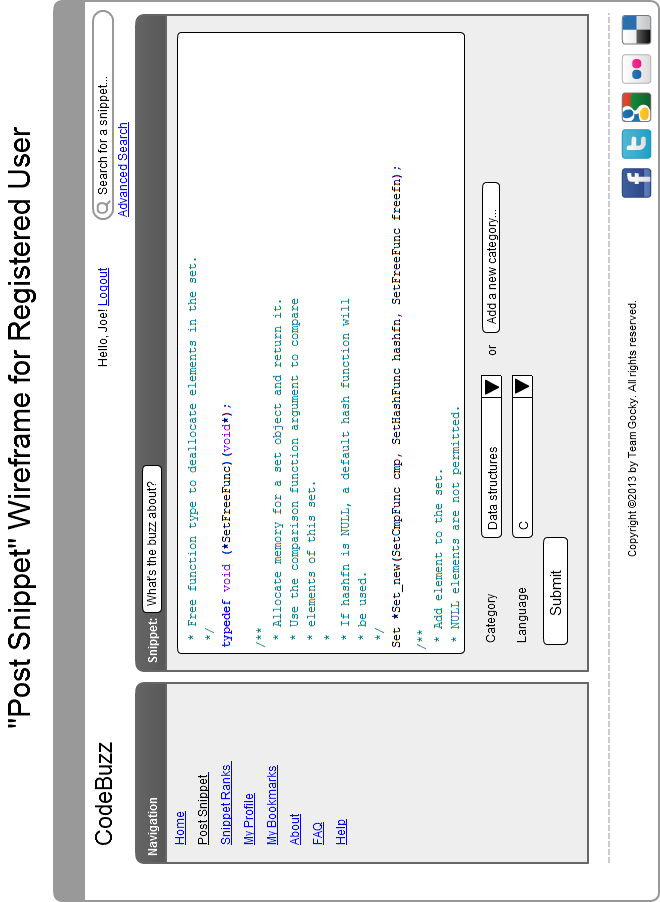
\includegraphics[width=\textwidth]{../imgs/CCodeSnippetHorz.png}
%\end{frame}

\end{document}
